\documentclass[a4paper,12pt]{report}

%Русский язык
\usepackage[T2A]{fontenc}
\usepackage[utf8]{inputenc}
\usepackage[english,russian]{babel}
\usepackage{cmap}

%Работа с кодом
\usepackage{listings}
\usepackage{color}

\definecolor{green}{rgb}{0,0.6,0}
\definecolor{gray}{rgb}{0.5,0.5,0.5}
\definecolor{red}{rgb}{0.6,0,0}

\lstset{
        language=Python, 
        basicstyle=\small\ttfamily, 
        numberstyle=\tiny,           
        columns=flexible,
        stepnumber=1,                   
        numbersep=5pt,        
        showspaces=false,
        showstringspaces=false,
        showtabs=false,
        tabsize=2,                
        captionpos=b,              
        breaklines=true,           
        breakatwhitespace=false,
        keywordstyle=\color{green},
        commentstyle=\color{gray},
        stringstyle=\color{red},      
}

%Математика
\usepackage{amsmath,amsfonts,amssymb,amsthm,mathtools} 

%Изображения
\usepackage{float}
\usepackage{graphicx}
\graphicspath{ {./img/} }

%Поля страницы
\usepackage{geometry} 
\geometry{left=2.3cm} 
\geometry{right=1.8cm} 
\geometry{top=2cm} 
\geometry{bottom=2.5cm} 

%Отступы
\usepackage{indentfirst}
\setlength{\parskip}{0cm}

\begin{document} 

\begin{titlepage}
\newpage
	\begin{center}
		\large Санкт-Петербургский политехнический университет Петра Великого\\
		Институт компьютерных наук и технологий\\
		Высшая школа интеллектуальных систем и суперкомпьютерных технологий\\
	\end{center}
\vspace{7cm}

\begin{center}
		\large \textbf{Отчёт по лабораторной работе №1} \\
		\textbf{Дисциплина:} Телекоммуникационные технологии\\
		\textbf{Тема:} Звуки и сигналы
\end{center}
\vspace{4cm}
	
\begin{flushright}
		\large Работу выполнил:\\ Ляшенко В.В.\\
		Группа: 3530901/80201\\
		Преподаватель:\\ Богач Н.В.
\end{flushright}

\vspace{\fill}
\begin{center}
	\large Санкт-Петербург\\ 2021
	\end{center}
\end{titlepage}

\tableofcontents
\listoffigures
\lstlistoflistings

\chapter{Упражнение 1.1}
    Создадим копию репозитория ThinkDSP и клонируем его на компьютер. Затем установим дистрибутив Anaconda, который содержит Jupyter Notebook. Теперь можно перейти к выполнению упражнений.
    
    В первом упражнении нам требуется для Jupyter загрузить \texttt{chap01.ipynb}, прочитать пояснения и запустить примеры.
    
    Все примеры были успешно запущены. В последнем примере при выставлении более низких значений \texttt{cutoff} звук получался более приглушённым (Рис.1.1).
\begin{figure}[H]
        \centering
        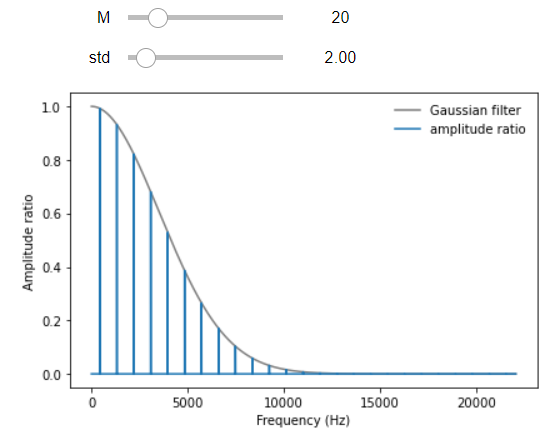
\includegraphics[width=0.8\textwidth]{fig1-1.PNG}
        \caption{Использование интерактивных виджетов IPython}
        \label{fig:fig1-1}
\end{figure}

\chapter{Упражнение 1.2}
\section{Сегмент}
    Скачаем с сайта \texttt{https://freesound.org} образец звука, имеющий чётко выраженную высоту. С помощью метода \texttt{read\_wave} прочтём запись. 
\begin{lstlisting}[caption=Чтение записи]
       from thinkdsp import read_wave
       wave = read_wave('sounds/564358__voxlab__chillout-vox-pad-chord-gb6.wav')
       wave.make_audio()
\end{lstlisting}

    Из этой записи выделим полусекундный сегмент, в котором высота постоянна (Рис.2.1).
\begin{lstlisting}[caption=Выделение сегмента]
       from thinkdsp import decorate
       segment = wave.segment(start=6, duration=0.5)
       segment.plot()
       decorate(xlabel='Time (s)')
\end{lstlisting}
\begin{figure}[H]
        \centering
        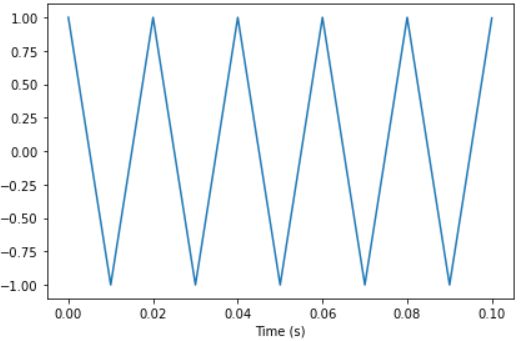
\includegraphics[width=0.8\textwidth]{fig2-1.PNG}
        \caption{Сегмент}
        \label{fig:fig2-1}
\end{figure}

\section{Спектр}
    После этого вычислим и распечатаем спектр выбранного сегмента (Рис.2.2).
\begin{lstlisting}[caption=Вычисление спектра]
       spectrum = segment.make_spectrum()
       spectrum.plot()
       decorate(xlabel='Frequency (Hz)')
\end{lstlisting}
\begin{figure}[H]
        \centering
        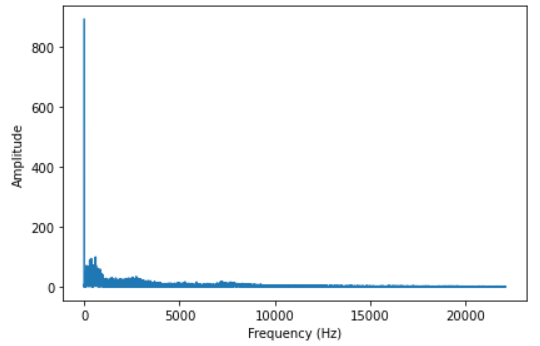
\includegraphics[width=0.8\textwidth]{fig2-2.PNG}
        \caption{Спектр}
        \label{fig:fig2-2}
\end{figure} 
 
    Тембр - это характеристика, определяющая восприятие качества звука. Тембр звука зависит от частот в спектре и их интенсивностей. Т.е. чем больше различных частот в спектре, тем богаче и насыщинее будет тембр.

\section{Фильтрация}
    Используем \texttt{high\_pass}, \texttt{low\_pass} и \texttt{band\_stop} для фильтрации гармоник.
\begin{lstlisting}[caption=Выполнение фильтрации]
       spectrum.high_pass(2000)
       spectrum.low_pass(10000)
       spectrum.band_stop(2050, 2950)
       spectrum.band_stop(3000, 5000)
       spectrum.band_stop(5050, 7950)
       spectrum.band_stop(8050, 9000)
       spectrum.plot(high=20000)
       decorate(xlabel='Frequency (Hz)')
\end{lstlisting}  

    На рис.2.3. видим результат фильтрации гармоник, полученный с помощью предложенных методов.

\begin{figure}[H]
        \centering
        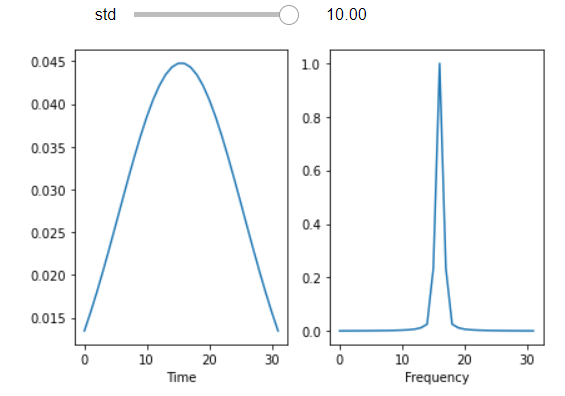
\includegraphics[width=0.8\textwidth]{fig2-3.PNG}
        \caption{Результат фильтрации}
        \label{fig:fig2-3}
\end{figure}

    Преобразуем спектр обратно в сигнал и послушаем его.
\begin{lstlisting}[caption=Преобразование спектра в сигнал]
       spectrum.make_wave().make_audio()
\end{lstlisting}      
  
    В результате фильтрации звук получился более тонким и звенящим.

\chapter{Упражнение 1.3}
\section{Сложный сигнал}
    Теперь создадим сложный сигнал из объектов \texttt{SinSignal} и
\texttt{CosSignal}, суммируя их. Полученный сигнал представлен на рис.3.1. Затем обработаем этот сигнал для получения \texttt{wave} и прослушаем его.
\begin{lstlisting}[caption=Создание сложного сигнала]
       from thinkdsp import CosSignal, SinSignal

       cos_sig1 = CosSignal(freq=250, amp=0.7, offset=0)
       sin_sig1 = SinSignal(freq=600, amp=0.4, offset=0)
       cos_sig2 = CosSignal(freq=350, amp=1.0, offset=0)
       sin_sig2 = SinSignal(freq=800, amp=0.8, offset=0)

       sum_sig = cos_sig1 + sin_sig1 + cos_sig2 + sin_sig2
       sum_sig.plot()
       decorate(xlabel='Time (s)')
       sum_sig.make_wave().make_audio()
\end{lstlisting}
\begin{figure}[H]
        \centering
        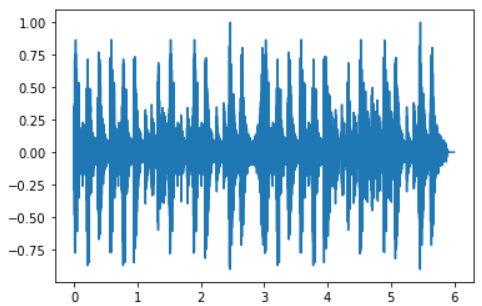
\includegraphics[width=0.8\textwidth]{fig3-1.PNG}
        \caption{Сложный сигнал}
        \label{fig:fig3-1}
\end{figure}

    Получившийся сигнал по звучанию похож на телефонный гудок.
    
\section{Спектр сложного сигнала}
    Вычислим спектр полученного сигнала и выведем его (Рис.3.2).
\begin{lstlisting}[caption=Вычисление спектра сложного сигнала]
       spectrum = sum_sig.make_wave().make_spectrum()
       spectrum.plot(1000)
       decorate(xlabel='Frequency (Hz)')
\end{lstlisting}
\begin{figure}[H]
        \centering
        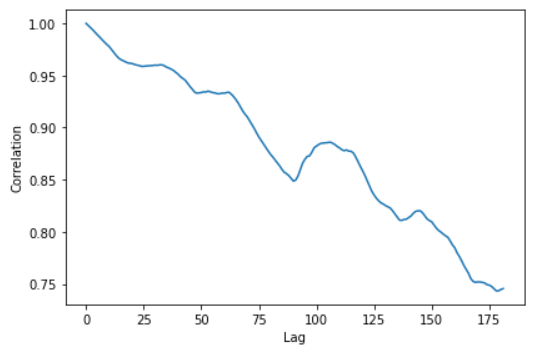
\includegraphics[width=0.8\textwidth]{fig3-2.PNG}
        \caption{Спектр сложного сигнала}
        \label{fig:fig3-2}
\end{figure}

\section{Некратные компоненты}
    Добавим частотные компоненты, не кратные основным.
\begin{lstlisting}[caption=Добавление новых компонентов]
       cos_sig3 = CosSignal(freq=3397, amp=0.6, offset=0)
       sin_sig3 = SinSignal(freq=2221, amp=0.9, offset=0)
       sum_sig = sum_sig + sin_sig3 + cos_sig3
       sum_sig.plot()
       decorate(xlabel='Time (s)')
       sum_sig.make_wave().make_audio()
\end{lstlisting}
\begin{figure}[H]
        \centering
        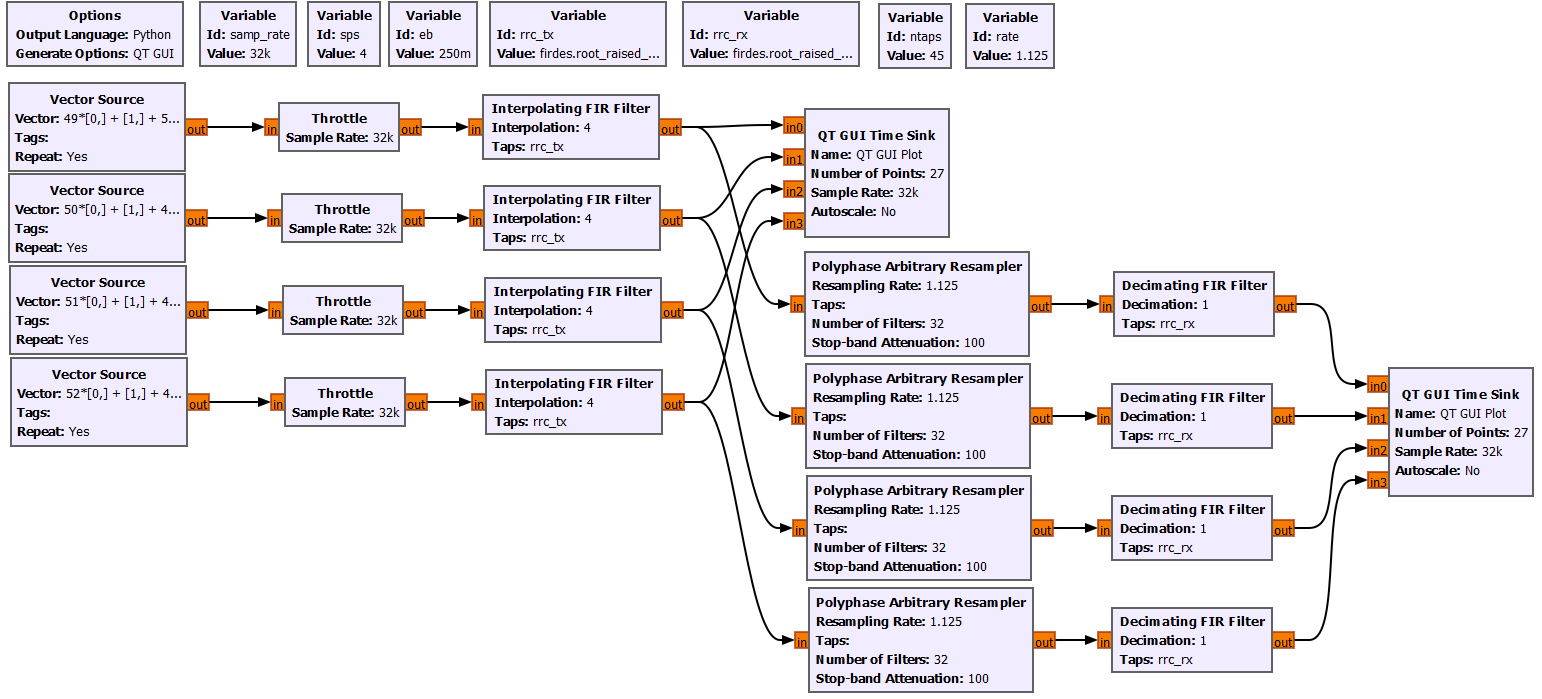
\includegraphics[width=0.8\textwidth]{fig3-3.PNG}
        \caption{Сложный сигнал с добавленными компонентами}
        \label{fig:fig3-3}
\end{figure}
    Получим спектр нового сигнала (Рис.3.4).
\begin{lstlisting}[caption=Вычисление спектра нового сигнала]
       spectrum = sum_sig.make_wave().make_spectrum()
       spectrum.plot(4000)
       decorate(xlabel='Frequency (Hz)')
\end{lstlisting}
\begin{figure}[H]
        \centering
        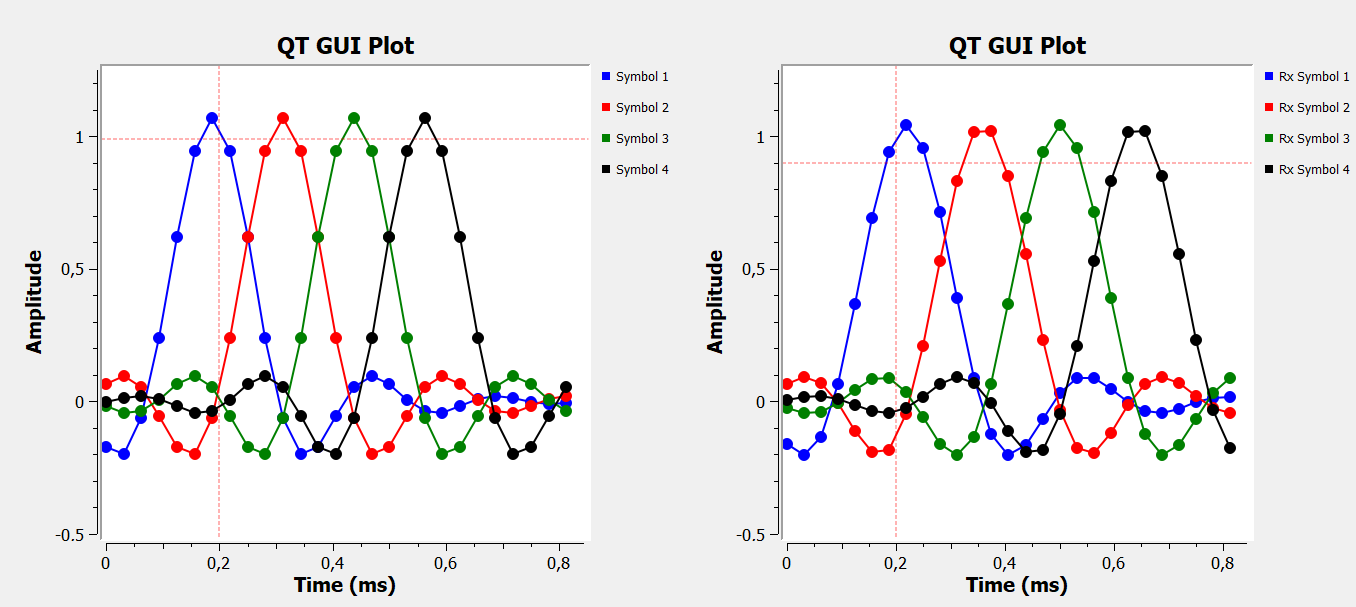
\includegraphics[width=0.8\textwidth]{fig3-4.PNG}
        \caption{Спектр нового сигнала}
        \label{fig:fig3-4}
\end{figure}   

    Получившийся звук стал более пищащим и неприятным.
    
\chapter{Упражнение 1.4}
    Напишем функцию \texttt{stretch}, которая будет ускорять или замедлять сигнал изменением \texttt{ts} и \texttt{framerate}.
\begin{lstlisting}[caption=Функция stretch]
       def stretch(wave, factor):
       wave.ts *= factor
       wave.framerate /= factor
\end{lstlisting} 
    
    Возьмём звук из Упражнения 1.2, создадим на его основе два сигнала и один из них замедлим, а другой ускорим (Рис.4.1-4.2).
\begin{lstlisting}[caption=Замедление сигнала]
       wave1 = read_wave('sounds/564358__voxlab__chillout-vox-pad-chord-gb6.wav')
       wave2 = read_wave('sounds/564358__voxlab__chillout-vox-pad-chord-gb6.wav')
       stretch(wave1, 2.0)
       wave1.plot()
       wave1.make_audio()
\end{lstlisting}
\begin{figure}[H]
        \centering
        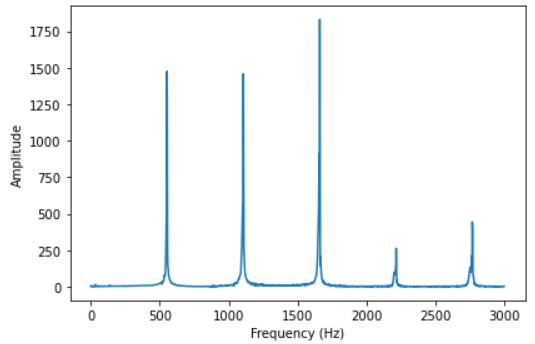
\includegraphics[width=0.8\textwidth]{fig4-1.PNG}
        \caption{Замедленный сигнал}
        \label{fig:fig4-1}
\end{figure} 

\begin{lstlisting}[caption=Ускорение сигнала]
       stretch(wave2, 0.2)
       wave2.plot()
       wave2.make_audio()
\end{lstlisting}
\begin{figure}[H]
        \centering
        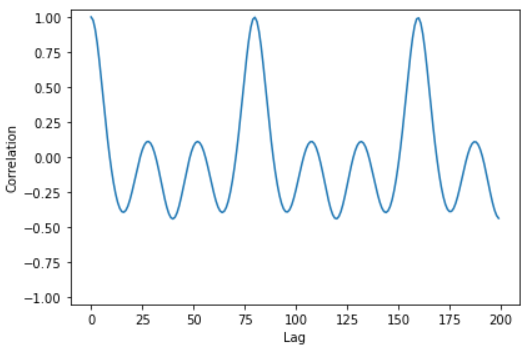
\includegraphics[width=0.8\textwidth]{fig4-2.PNG}
        \caption{Ускоренный сигнал}
        \label{fig:fig4-2}
\end{figure} 
  
    В первом случае звук стал более тяжёлым, он словно слышен через толщу воды. Во втором же случае звук наоборт стал писклявым и звенящим.

\chapter{Выводы}
    В результате выполнения данный работы мы познакомились с понятиями сигнала и звука, а также понятиями описывающими их. Кроме того, мы научились работать с сигналами, спектрами и звуковыми волнами, применяя различные функции, написанные на языке Python.
\end{document}